
\documentclass{beamer}

\usepackage{algpseudocode, color, colortbl}

\usepackage{hyperref}
\hypersetup{
    colorlinks=true,
    urlcolor=blue,
}

\usetheme{Montpellier}
\usecolortheme{rose}

% page numbers, from
% https://tex.stackexchange.com/questions/137022/how-to-insert-page-number-in-beamer-navigation-symbols
\expandafter\def\expandafter\insertshorttitle\expandafter{%
  \insertshorttitle\hfill%
  \insertframenumber\,/\,\inserttotalframenumber}

\definecolor{Gray}{gray}{0.8}
\newcolumntype{g}{>{\columncolor{Gray}}c}

\newcommand{\stanza}{ \\~\ }

\title{05. Linear-Time Sorting and Selection}
\subtitle{CPSC 535}
\author{Kevin A. Wortman}
\institute{ 
\includegraphics[height=2cm]{csuf-logo-cmyk} }
\date{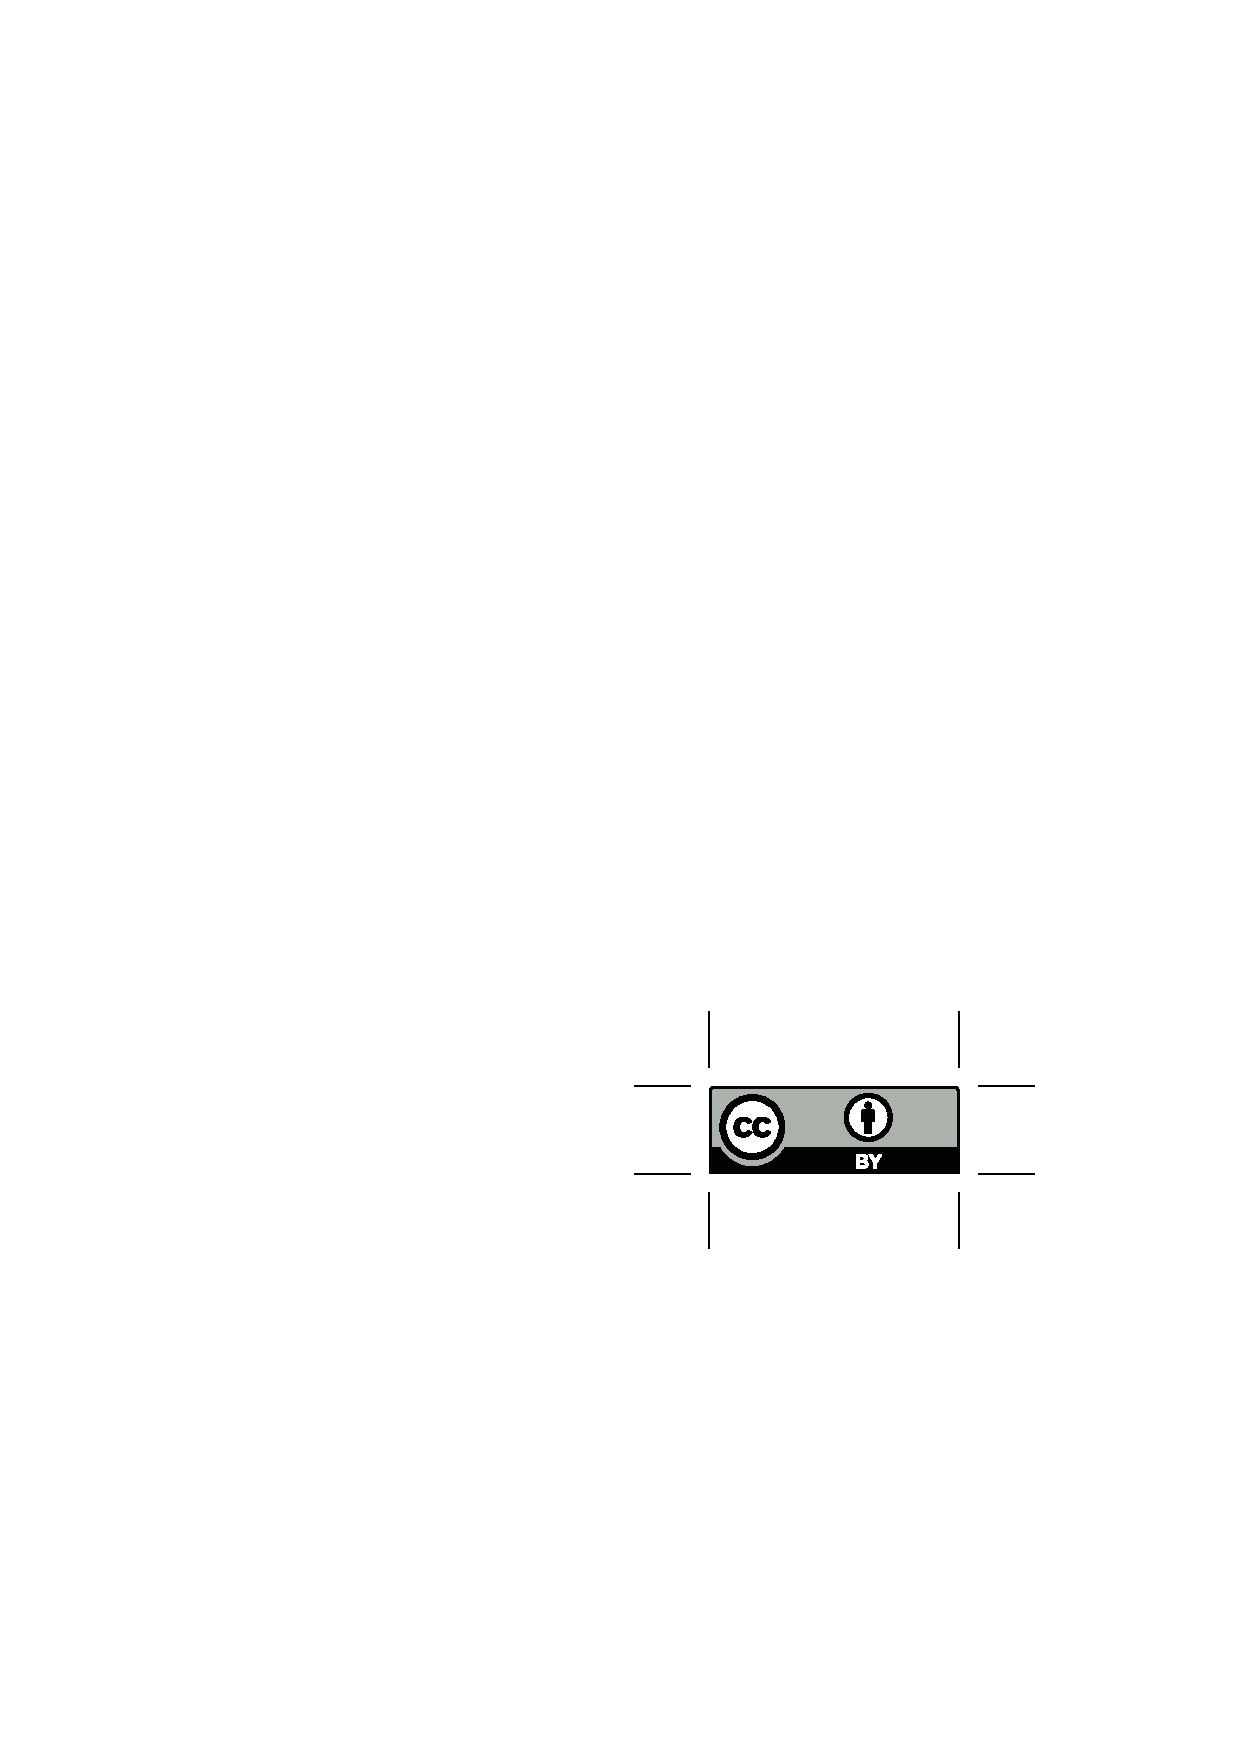
\includegraphics[height=14pt]{by} \\

{\tiny
This work is licensed under a
\href{http://creativecommons.org/licenses/by/4.0/}{Creative Commons Attribution 4.0 International License}.
}}

\begin{document}

\begin{frame}
  \titlepage
\end{frame}

\begin{frame} \frametitle{Big Idea in Computer Science}

\textbf{``What is old is new again''}: CS principles are solved science; society's
needs, economic factors, and fads dictate which are prominent and which are in the background

\begin{itemize}
  \item thin clients dominated the mainframe era; thick clients
    dominated the PC era; thin clients dominate the web app era
  \item memory conservation was critical prior to the 90s;
    programmer labor was more important, until mobile phones
  \item Unix rose (70s), fell (80s-90s), rose again (MacOS, iOS, Android,
    ChromeOS, Linux, PlayStation, embedded)
  \item algorithms were considered ivory-tower theory until recently
\end{itemize}

\textbf{Protip:}  the CS material that seems irrelevant now, will probably
become extremely marketable later in your career
\end{frame}

\begin{frame} \frametitle{Big Idea in Algorithm Design}

\textbf{Paramaterized complexity}: algorithm complexity measured both in terms
of input size $n$, \textbf{and} some parameter describing the values in the input
\begin{itemize}
  \item machine word size $W$ (e.g. $W=64$ on modern PCs)
  \item \# distinct values $k$
\end{itemize}

\textbf{Pseudopolynomial}: polynomial over both $n$, and also parameters
\begin{itemize}
  \item radix sort takes $\Theta(nW)$ time
  \item strictly speaking $W$ could be as large as $n$, so $\Theta(nW)=\Theta(n^2)$, unimpressive
  \item in practice all real-world computers have $W \in \Theta(1)$ so $\Theta(nW)=\Theta(n)$,
    faster than $\Theta(n \log n)$
  \item arguably defying the spirit of the Random Access Model
\end{itemize}

\textbf{Tool to circumvent} lower bounds, $NP$-hardness
\end{frame}

\begin{frame} \frametitle{The Lower Bound for the Sorting Problem}

Recall the precise phrasing of the theorem: \\
\emph{Any comparison sort algorithm requires $\Omega(n \log n)$ comparisons
 in the worst case.} \stanza

Bad news: $O(n \log n)$ ``speed limit'' for this important problem \stanza

Good news:
\begin{itemize}
  \item optimal $\Theta(n \log n)$-time algorithms: mergesort, heapsort, quicksort
  \item loophole: theorem only applies to ``comparison sorts''
  \item loophole: theorem applies to the general sorting problem, but we could
    make the problem more specific
\end{itemize}
\end{frame}

\begin{frame} \frametitle{Counting Sort Problem}
Recall the classical \emph{sorting problem:} \\
\textbf{input:} a sequence of $n$ numbers $A=\langle a_1, a_2, \ldots, a_n \rangle$ \\
\textbf{output:} a permutation (reordering) $\langle a_1', a_2', \ldots, a_n' \rangle$
  of the input sequence such that $a_1' \leq a_2' \leq \ldots, a_n'.$ \stanza

What if the inputs $a_i$ are all bounded integers? \stanza

\emph{counting sort problem:} (changes are \underline{underlined}) \\
\textbf{input:} \underline{an integer $k \geq 0$, and}
  a sequence of $n$ \underline{integers} $A=\langle a_1, a_2, \ldots, a_n \rangle$,
  \underline{where each $a_i \in [0, k]$} \\
\textbf{output:} same \stanza

Turns out this change admits a $\Theta(n)$-time algorithm.
\end{frame}

\begin{frame} \frametitle{Counting Sort Idea}
\begin{itemize}
  \item each $a_i$ can work as an array index
  \item count the number of occurrences of each value; create array $C$ where
    \[ C[x] = \text{ the number of times that } x \text{ appears in A } \]
  \item let $B$ be the output array
  \item use the counts in $C$ to plan out which indices of $B$ will hold each $a_i$
  \item fill in $B$ using this information
\end{itemize}
\end{frame}

\begin{frame} \frametitle{Counting Sort Pseudocode}
  \begin{algorithmic}[1]
    \Function{COUNTING-SORT}{A, B, k}
    \State allocate new array $C[0, \ldots, k]$, initialized to all zeroes
    \For {$j$ from 1 to $A.length$}
      \State $C[A[j]]++$ \Comment{ $C[i]$ is the number of elements $=i$ }
    \EndFor
    \For {$i$ from 1 to $k$}
      \State $C[i] += C[i-1]$ \Comment{ $C[i]$ is the number of elements $\leq i$ }
    \EndFor
    \For { $j$ from $A.length$ down to 1 }
      \State $B[C[A[j]]] = A[j]$
      \State $C[A[j]]--$
    \EndFor
    \EndFunction
  \end{algorithmic}
\end{frame}

\begin{frame} \frametitle{Counting Sort Analysis}
\begin{itemize}
  \item allocate $C$: $\Theta(k)$ time
  \item first \textbf{for} loop: $\Theta(n)$ time
  \item second \textbf{for} loop: $\Theta(k)$ time
  \item third \textbf{for} loop: $\Theta(n)$ time
  \item total = $\Theta(k+n+k+n)=\Theta(2k+2n)=\Theta(k+n)$ time
\end{itemize}
\end{frame}

\begin{frame} \frametitle{When Counting Sort Wins}
  If $k \in O(n)$, then counting sort takes $\Theta(k+n)=\Theta((n)+n)=\Theta(n)$ time. \stanza

Applications where $k \ll n$
\begin{itemize}
\item DNA sequences have only $k=4$ bases A, C, G, T; human genome has $n \approx 3$ billion bases
\item $n$-character ASCII string has only $k=127$ character values
\item log of website analytics has $n$ hits but only $k$ distinct web page URLs;
  each page is visited many times so $n \gg k$
\end{itemize}
\end{frame}

\begin{frame} \frametitle{When Counting Sort Loses}
In the general sorting problem, each $a_i$ is unbounded, so the maximum element
could use $\Theta(n)$ bits, have value
\[ a_i = 2^n = k \]
and force counting sort to take
\[ \Theta(k+n)=\Theta((2^n)+n)=\Theta(2^n) \]
time, which is \textbf{exponential} in $n$ and much more expensive than
$\Theta(n \log n)$ \stanza

$\implies$ counting sort is optimal when the software designer knows that the
input is always a set of $k$ integers with $k \in O(n)$ \stanza

$\implies$ \textbf{but} if that is not guaranteed, comparison sorts are still optimal
\end{frame}

\begin{frame} \frametitle{Stable Sorting}
\textbf{stable} sorting algorithm: does not swap order of ties \stanza

if $a_i=a_j$ and $i<j$ then $i' < j'$ \stanza

Ex.: suppose we sort
\[ [(47, a), (13, c), (28, b), (13, d)] \]
by the first element of each pair; a \emph{stable} sort guarantees $(13, c)$
comes before $(13, d)$ \stanza

Stability is a convenient, desirable property \stanza

Stable: insertion sort, mergesort, counting sort \\
Not stable: heapsort, quicksort
\end{frame}

\begin{frame} \frametitle{``Radix''}
Vocabulary quiz:
\begin{itemize}
  \item what does \textbf{radix} mean?
  \item where else do we use the word ``radix''?
\end{itemize}
\end{frame}

\begin{frame} \frametitle{Radix Sort Overview}
\begin{itemize}
  \item make counting sort more robust to large elements
  \item sort one digit at a time
  \item i.e. sort by least-significant-digit, then by second-least-significant-digit, $\ldots$,
    sort by most-significant digit
  \item e.g. to sort names in a spreadsheet: sort by first name, then by last name
  \item originally
  \href{https://en.wikipedia.org/wiki/Radix_sort\#/media/File:SEACComputer_038.jpg}{used by pre-digital punchcard sorting machines}
    (what's old...)
  \item now used for parallel sort in GPU (...is new again)
\end{itemize}
\end{frame}

\begin{frame} \frametitle{Radix Sort Worked Example}
\begin{center}
(Sorting one base-10 digit at a time.)
\begin{columns}
\begin{column}{0.25\textwidth}
  \begin{center}
    \begin{tabular}{ccg}
      7&7&5 \\
      0&5&3 \\
      7&6&2 \\
      7&9&1 \\
      6&7&4 \\
      5&2&1 \\
      3&3&4 \\
      2&2&5 \\
    \end{tabular}
  \end{center}
\end{column}
\begin{column}{0.25\textwidth}
  \begin{center}
    \begin{tabular}{cgc}
      7&9&1 \\
      5&2&1 \\
      7&6&2 \\
      0&5&3 \\
      6&7&4 \\
      3&3&4 \\
      7&7&5 \\
      2&2&5 \\
    \end{tabular}
  \end{center}
\end{column}
\begin{column}{0.25\textwidth}
  \begin{center}
    \begin{tabular}{gcc}
      5&2&1 \\
      2&2&5 \\
      3&3&4 \\
      0&5&3 \\
      7&6&2 \\
      6&7&4 \\
      7&7&5 \\
      7&9&1 \\
    \end{tabular}
  \end{center}
\end{column}
\begin{column}{0.25\textwidth}
  \begin{center}
    \begin{tabular}{gcc}
      0&5&3 \\
      2&2&5 \\
      3&3&4 \\
      5&2&1 \\
      6&7&4 \\
      7&6&2 \\
      7&7&5 \\
      7&9&1 \\
    \end{tabular}
  \end{center}
\end{column}
\end{columns}
\end{center}
\end{frame}

\begin{frame} \frametitle{Radix Sort, 1 bit at a time}
  \begin{algorithmic}[1]
    \Function{RADIX-SORT-1}{A, W}
    \For {$i$ from 1 to $W$}
      \State use a stable sort to sort $A$ based only on
        bit position $i$
    \EndFor
    \EndFunction
  \end{algorithmic}
  \vspace{.5cm}

Using counting sort as the stable sort, we have $k=2$ (bit values 0 or 1) so each
loop iteration takes $\Theta(k+n)=\Theta(2+n)=\Theta(n)$ time \stanza

Clearly $W$ iterations $\implies \Theta(nW)$ total time
\end{frame}

\begin{frame} \frametitle{Radix Sort, 8 bits at a time}
  \begin{algorithmic}[1]
    \Function{RADIX-SORT-8}{A, W}
    \For {$i$ from 1 to $\lceil W/8 \rceil$}
      \State stably sort $A$ on bits $8i-7$ through $8i$
    \EndFor
    \EndFunction
  \end{algorithmic}
  \vspace{.5cm}

$k=2^8=256 \in \Theta(1)$ \\
number of iterations is $\lceil nW/8 \rceil \in \Theta(n)$ \\
$\implies$ still $\Theta(nW)$ time, but with different constant factors \stanza

Let $r=$\#bits per pass; optimal choice of $r$ minimizes
\[ \lceil W/r \rceil \cdot (2^r + n) \]
\end{frame}

\begin{frame} \frametitle{Minimum and Maximum}
  \begin{algorithmic}[1]
    \Function{MINIMUM}{A}
    \State min = A[1]
    \For {$i$ from 2 to $A.length$}
      \If {$min > A[i]$}
        \State $min = A[i]$
      \EndIf
    \EndFor
    \State \Return{ $min$ }
    \EndFunction
  \end{algorithmic}
  \vspace{.5cm}

  $\Theta(n)$ time \stanza

  can also find maximum in $\Theta(n)$ time, or both in $\Theta(n)$ time
\end{frame}

\begin{frame} \frametitle{Selection Problem and Baseline Algorithm}
\textbf{input:} array of $n$ numbers $A=\langle a_1, a_2, \ldots, a_n \rangle$;
  index $i \in \{1, 2, \ldots, n\}$\\
\textbf{output:} the $i$th smallest element of $A$ \stanza

\begin{algorithmic}[1]
  \Function{SELECTION-BY-SORTING}{A, i}
  \State \Return{ $MERGE-SORT(A)[i]$ }
  \EndFunction
\end{algorithmic}
\vspace{.5cm}
Clearly $\Theta(n \log n)$ time \stanza

\textbf{Surprise:} selection can be solved in only $\Theta(n)$ time
\end{frame}

\begin{frame} \frametitle{Randomized Quicksort Review}
\begin{columns}
\begin{column}{0.5\textwidth}
  \begin{algorithmic}[1]
    \Function{RQSORT}{A, p, r}
    \If { $p < r$ }
      \State $q = RPART(A, p, r)$
      \State $RQSORT(A, p, q-1)$
      \State $RQSORT(a, q+1, r)$
    \EndIf
    \EndFunction
  \end{algorithmic}
  \vspace{.5cm}
  Non-stable sort in $\Theta(n \log n)$ expected time but
  $\Theta(n^2)$ worst-case time
\end{column}
\begin{column}{0.5\textwidth}
  \begin{algorithmic}[1]
    \Function{RPART}{A, p, r}
    \State $i = $ random in $[p, r]$
    \State $swap(A[i], A[r])$
    \State $pivot = A[r]$
    \State $i = p$
    \For { $j$ from $p$ to $r-1$ }
      \If { $A[j] < pivot$ }
        \State $swap(A[i], A[j])$
        \State $i++$
      \EndIf
    \EndFor
    \State $swap(A[i], A[r])$
    \State \Return{ $i$ }
    \EndFunction
  \end{algorithmic}
\end{column}
\end{columns}
\end{frame}

\begin{frame} \frametitle{Randomized Selection Overview}
\begin{itemize}
  \item combining ideas from binary search and quicksort
  \item recursively search for $i$th smallest element
  \item do randomized partition; then
  \item three cases
    \begin{itemize}
      \item pivot happens to be $i$th smallest
      \item need to keep searching before pivot
      \item need to keep searching after pivot
    \end{itemize}
  \item expected runtime is $T(n) \approx T(n/2) + \Theta(n)$
  \item counterintuitively, that solves to $\Theta(n)$
  \end{itemize}
\end{frame}

\begin{frame} \frametitle{Randomized Selection Pseudocode}
  \begin{algorithmic}[1]
    \Function{RSELECT}{A, p, r, i}
    \If { $p==r$ }
      \State \Return{ $A[p]$ } \Comment{ base case, done }
    \EndIf
    \State $q = RPART(A, p, r)$ \Comment{ partition, $q$ is pivot index }
    \State $k = q - p + 1$ \Comment{ $k =$ number of elements before pivot }
    \If { $i==k$ }
      \State \Return{ $A[q]$ } \Comment{ pivot is answer }
    \ElsIf { $i < k $ }
      \State \Return { $RSELECT(A, p, q-1, i)$ }
    \Else
      \State \Return { $RSELECT(A, q+1, r, i-k)$ } \Comment{$i$ decreases by $k$}
    \EndIf
    \EndFunction
  \end{algorithmic}
\end{frame}

\begin{frame} \frametitle{Randomized Selection Analysis}
\begin{itemize}
  \item at most one recursive call, on $n/2$ elements on average
  \item partitioning takes $\Theta(n)$ time
  \item rest of algorithm takes $\Theta(1)$ time
  \item expected running time
    \[ T(n) = T(n/2) + \Theta(n) \]
    which is only $\Theta(n)$ by master theorem
  \item worst case is the same for quicksort, extreme pivot at each step,
    $\Theta(n^2)$ time
  \item \textbf{takeaway:} randomized selection takes $\Theta(n)$ expected time
    and $\Theta(n^2)$ worst-case time
  \end{itemize}
\end{frame}

\begin{frame} \frametitle{Deterministic Selection Overview}
\begin{itemize}
  \item \textbf{deterministic:} perfectly predictable; not randomized
  \item recall that $T(n) = T(fn) + \Theta(n)$ is $\Theta(n)$ for any fraction $0<f<1$,
    not just $f=1/2$
  \item need: deterministic process to find a not-terrible pivot
  \item i.e. need at least $fn$ elements on each side of the pivot, so that
    the worst-case recursive call is $T((1-f)n)$
  \item e.g. need at least $\frac{1}{3}n$ elements on each side of the pivot,
    so that there is a $T(\frac{1}{3}n)$ or $T(\frac{2}{3}n)$ call;
    worst-case is $T(\frac{2}{3}n)$; so
    \[ T(n)=T(\frac{2}{3}n) + \Theta(n) \]
    which is still $\Theta(n)$ (though with worse constants)
\end{itemize}
\end{frame}

\begin{frame} \frametitle{Deterministic Selection Process}
\begin{enumerate}
  \item divide $n$ elements into $\approx n/5$ groups of 5 elements each
  \item find the median of each group with $SELECTION-BY-SORTING$;
    $\Theta(n(5 \log 5))=\Theta(n)$ time
  \item form a new array of the medians, and recursively select the median
    of this array $=$ ``median-of-medians''; $T(n/5)$ time
  \item partition as usual, using median-of-medians as the pivot; $\Theta(n)$ time
  \item same three cases: either pivot is answer, or recurse before pivot, or
    recurse after pivot; $T(\text{max. \# elements on either side of pivot})$
\end{enumerate}
\end{frame}

\begin{frame} \frametitle{Deterministic Selection Analysis}
\begin{itemize}
  \item let $x$ be the median-of-medians; count elements $\geq x$
  \item suppose W.L.O.G. that input elements are distinct
  \item $\therefore$ at least half of the group-medians are $\geq x$
  \item $\therefore$ at least half of the groups contain at least 3 elements $\geq x$ each;
    except for the group containing $x$, and possibly one group with $<5$ elements
  \item $\therefore$ \#elements $\geq x$ is at least
  \[ 3 \Big( \Big\lceil \frac{1}{2} \lceil \frac{n}{5} \rceil \Big\rceil -2 \Big)
     \geq \frac{3}{10}n - 6 \]
  \item symmetrically there are at least $\frac{3}{10}n-6$ elements $\leq x$
  \item $\therefore$ recursively select at most $n-(\frac{3}{10}n-6)=\frac{7}{10}n+6$ elements
\end{itemize}
\end{frame}

\begin{frame} \frametitle{Deterministic Selection Analysis (continued)}
For some $t \in \Theta(1),$
  \[ T(n) \leq
      \begin{cases}
        O(1) & n < t \\
        T(\lceil n/5 \rceil) + T(\frac{7}{10}n+6) + O(n) & n \geq t .
      \end{cases}
  \]

The master theorem does not apply, but the substitution method can be used to
show $T(n) \in O(n).$ \stanza

\textbf{Takeaway:} Deterministic selection takes $O(n)$ worst-case time. \stanza

Surprise: selection can be \textbf{derandomized}
from $O(n)$ expected time to $O(n)$ worst-case time with no asymptotic overhead. \stanza

Impractical; much worse constant factors, not usually worth it.
\end{frame}

\end{document}
